\documentclass[shortpres]{beamer}
\usetheme{CambridgeUS}

% Depending on build configuration, one of these packages will
% enable unicode
%\usepackage[utf8]{inputenc}
\usepackage{fontspec}


%Images
\usepackage{graphicx, svg}
\usepackage{caption}

%Showing movies and gifs
%\usepackage{animate, media9, movie15}
\usepackage{animate}
\usepackage{array}
\usepackage{subfig}
\usepackage{multicol}
\usepackage{color}
\usepackage{pgfplots}
\usepackage{xmpmulti}

\usepackage{algorithm,algpseudocode}  %for algorithm environment

\setbeamertemplate{footline}
{
	\leavevmode%
	\hbox{%
		\begin{beamercolorbox}[wd=.333333\paperwidth,ht=2.25ex,dp=1ex,center]{author in head/foot}%
			\usebeamerfont{author in head/foot}\insertshortauthor%~~\beamer@ifempty{\insertshortinstitute}{}{(\insertshortinstitute)}
		\end{beamercolorbox}%
		\begin{beamercolorbox}[wd=.333333\paperwidth,ht=2.25ex,dp=1ex,center]{title in head/foot}%
			\usebeamerfont{title in head/foot}\insertshorttitle
		\end{beamercolorbox}%
		\begin{beamercolorbox}[wd=.333333\paperwidth,ht=2.25ex,dp=1ex,right]{date in head/foot}%
			\usebeamerfont{date in head/foot}\insertshortdate{}\hspace*{2em}
			\insertframenumber{} / \inserttotalframenumber\hspace*{2ex}
	\end{beamercolorbox}}%
	\vskip0pt%
}\part{title}
\beamertemplatenavigationsymbolsempty


%color specification---------------------------------------------------------------
\definecolor{TUMblue}{rgb}{0.00, 0.40, 0.74}
\definecolor{TUMgray}{rgb}{0.85, 0.85, 0.86}
\definecolor{TUMpantone285C}{rgb}{0.00, 0.45, 0.81}
\definecolor{lightblue}{rgb}{0.7529,0.8118,0.9333}

\setbeamercolor{block title}{fg=white, bg=TUMpantone285C}
\setbeamercolor{block body}{bg=lightblue}
\setbeamertemplate{blocks}[rounded][shadow=true]
%----------------------------------------------------------------------------------

\setbeamercolor{frametitle}{fg=TUMblue, bg=white}
\setbeamercolor{palette primary}{fg=TUMblue,bg=TUMgray}
\setbeamercolor{palette secondary}{use=palette primary,fg=TUMblue,bg=white}
\setbeamercolor{palette tertiary}{use=palette primary,fg=white, bg=TUMblue}
\setbeamercolor{palette quaternary}{use=palette primary,fg=white,bg=TUMpantone285C}


\setbeamercolor{title}{bg=white,fg=TUMblue}
\setbeamercolor{item projected}{use=item,fg=black,bg = lightblue}
\setbeamercolor{block title}{fg=black, bg=lightblue}
\setbeamercolor{block body}{bg=white}
\setbeamertemplate{blocks}[rounded][shadow=true]
%----------------------------------------------------------------------------------



%############### Self defined commands ##############################
\newcommand{\imgvoffset}{-20pt}
\newcommand{\texthoffset}{20pt}
\newcommand{\imgfullscale}{0.75}

\captionsetup[subfigure]{labelformat=empty}		%Disable enumeration of subfigures
%####################################################################

\usepackage{anyfontsize}

\title[{Tsunami simulation}]{Assignment 2}

\author[Bellamy, Honal, Wieser]{Gruppe XX\\George Bellamy, Christoph Honal, Felix Wieser\\\vspace{10pt}{\small Bachelorpraktikum}}

\institute[TU M\"unchen]{Technical University of Munich}

\date{21. November 2017}

\begin{document}
\maketitle

\begin{frame}{Demonstration of bathymetry}
	\begin{figure}
		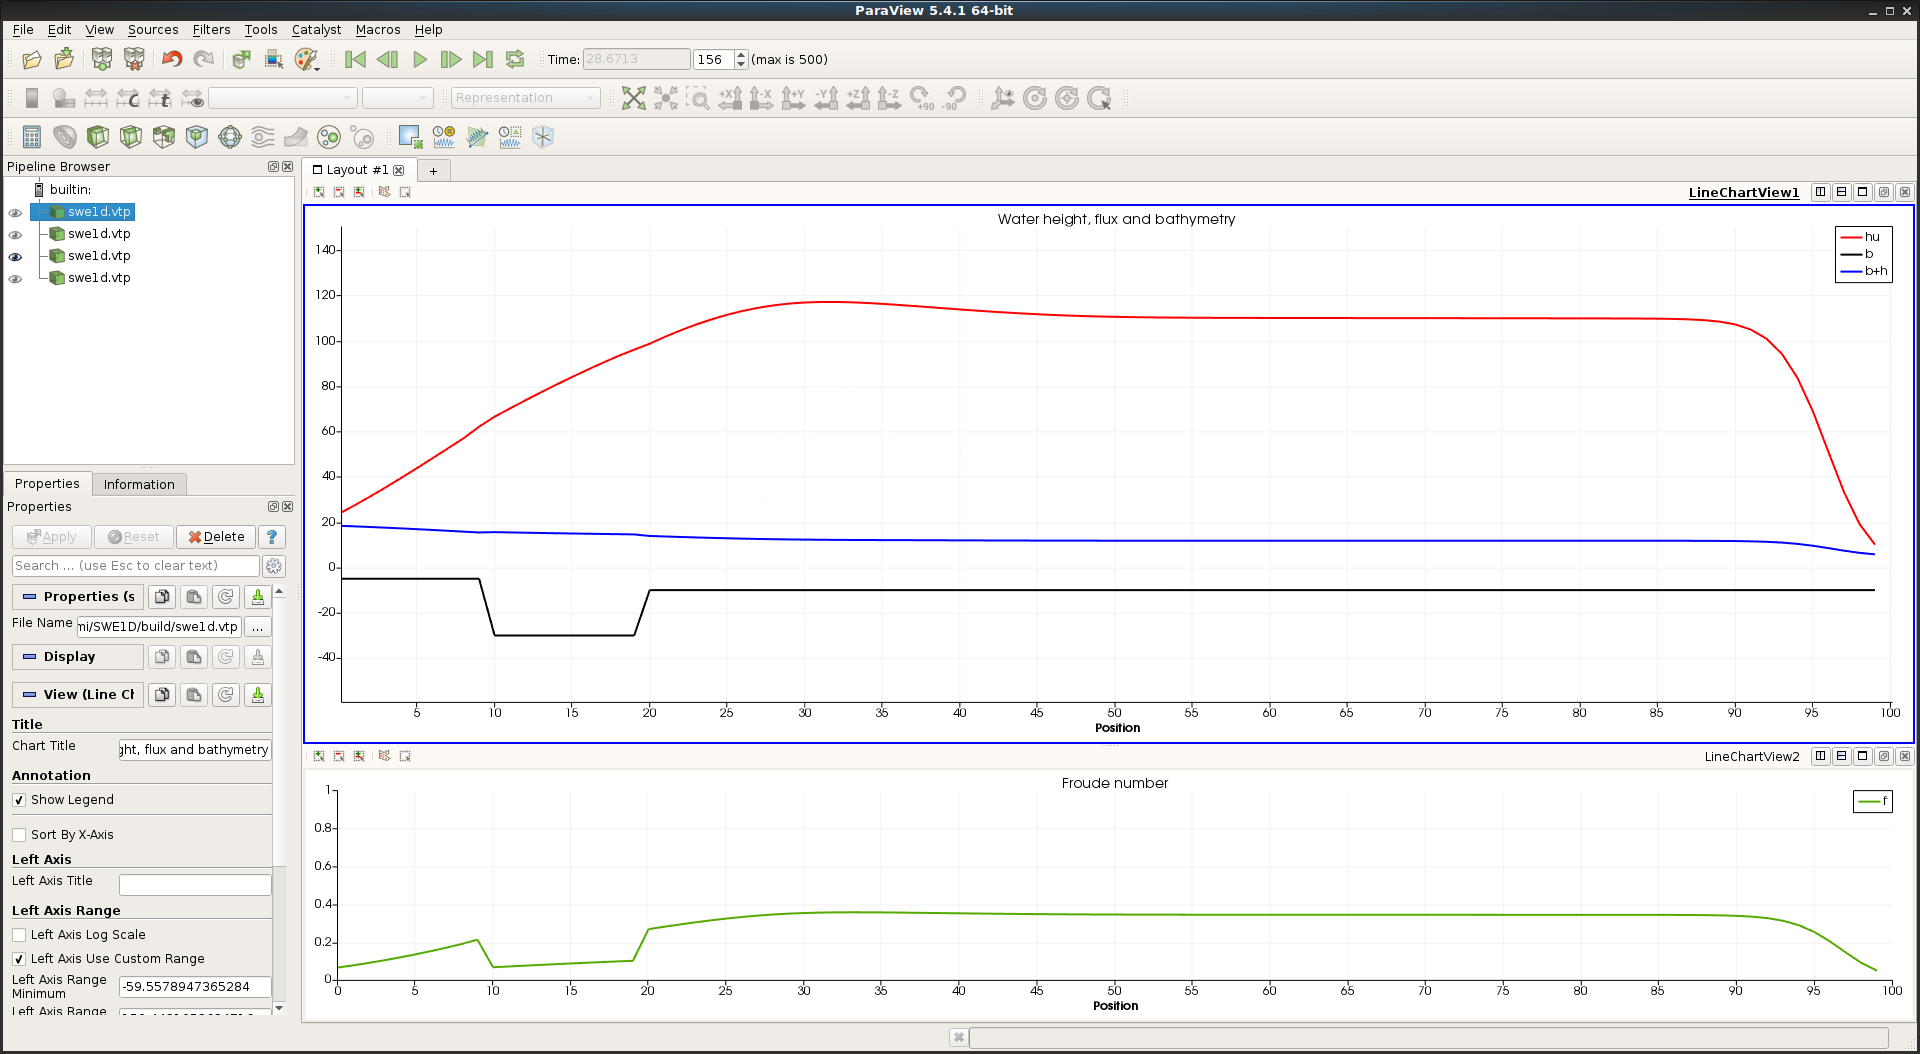
\includegraphics[clip, width=\imgfullscale\linewidth]{img/Bathymetry_simple.png}
	\end{figure}
	Reaction of the water stream to bathymetrie with constant water height\\
	Bump in froude number
\end{frame}

\begin{frame}{One-sided shock-shock problem}
	\begin{figure}
		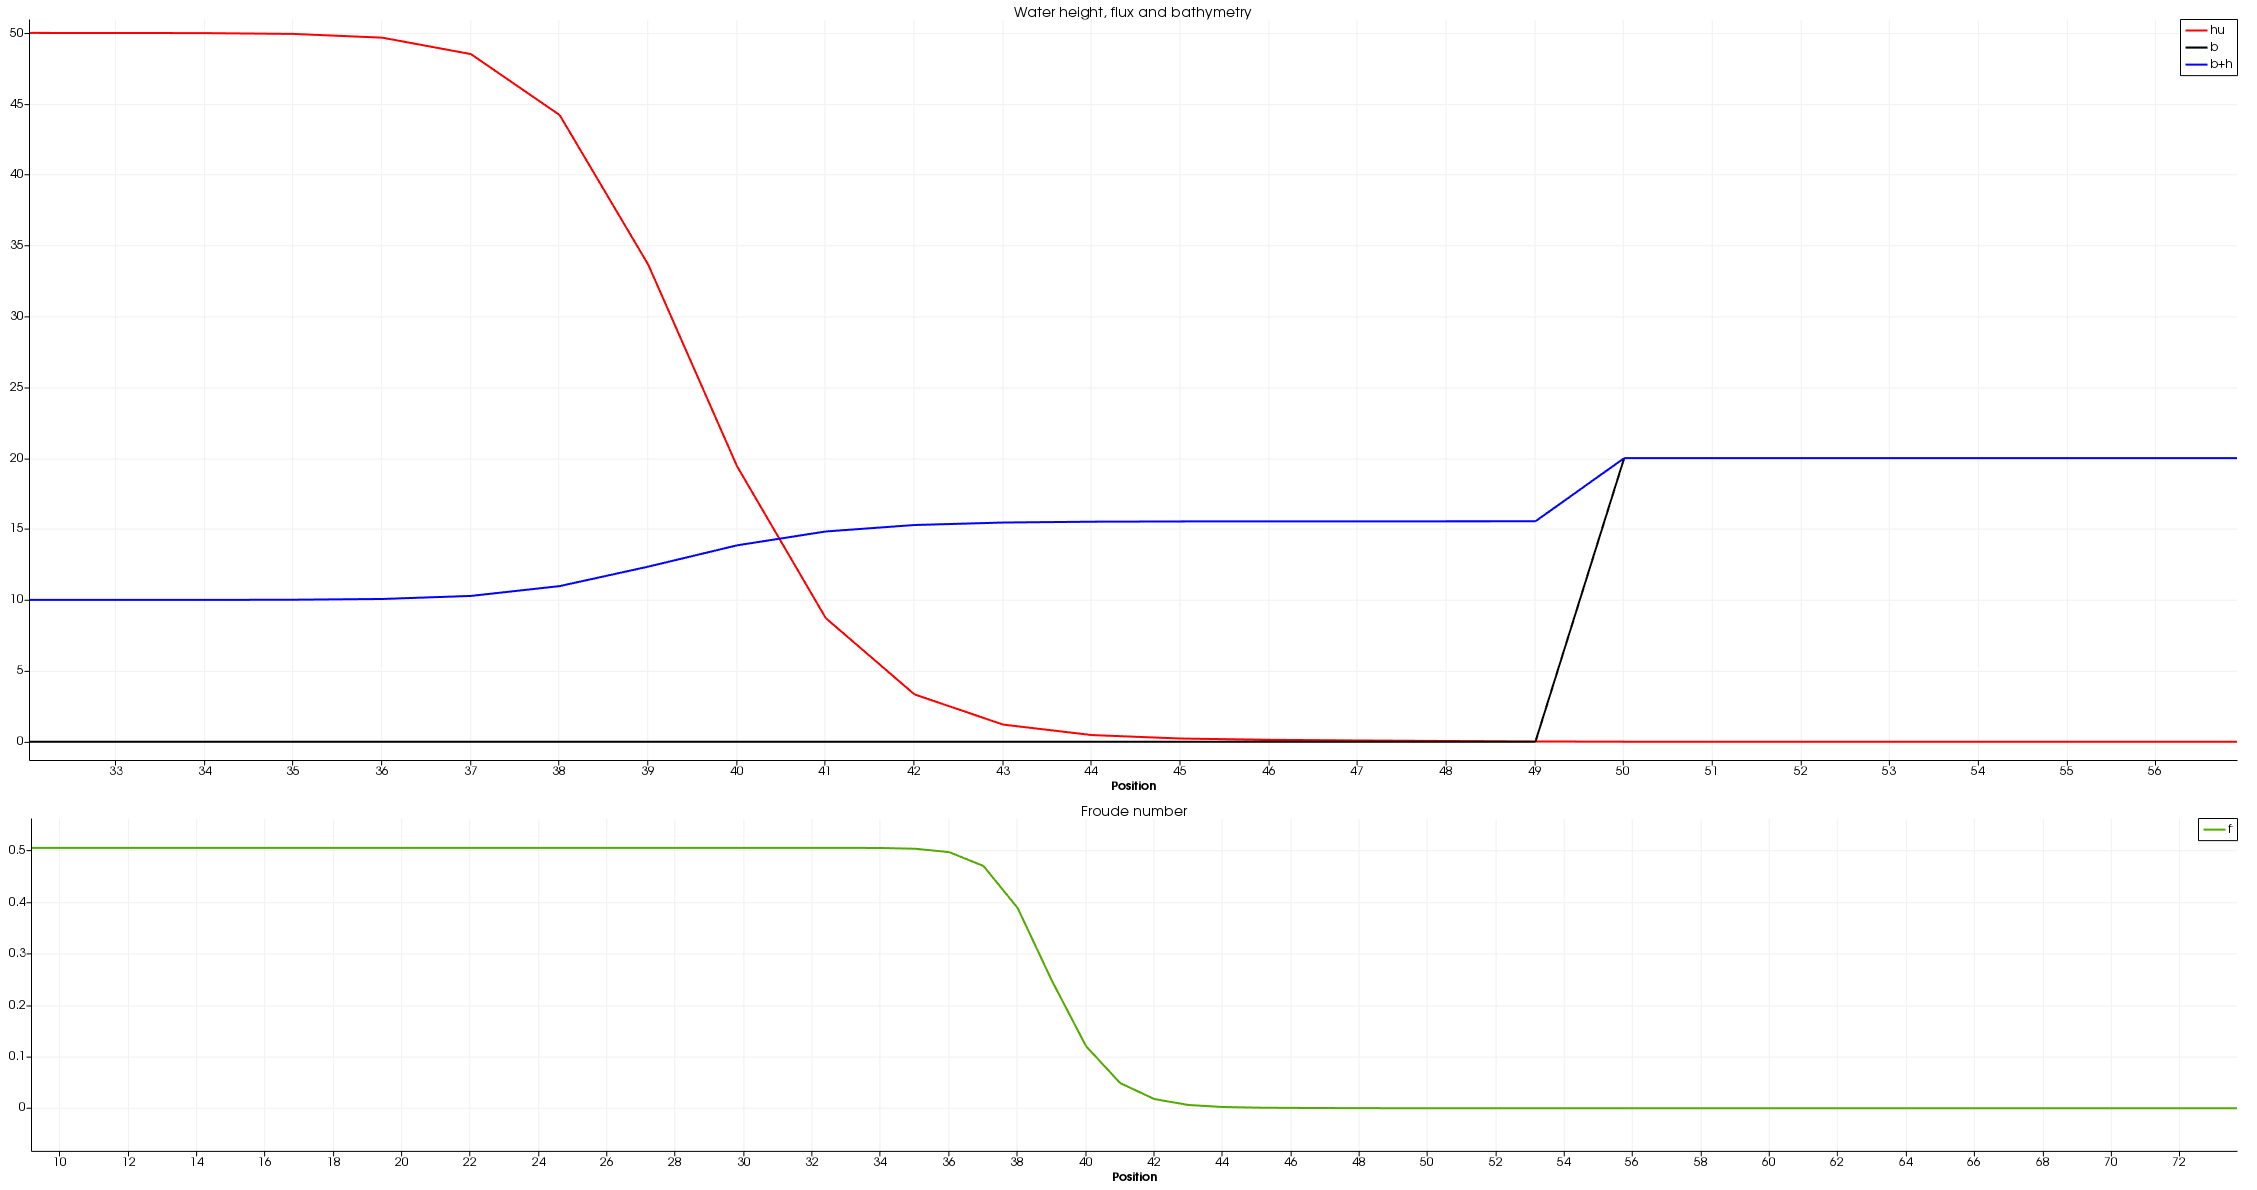
\includegraphics[clip, width=\imgfullscale\linewidth]{img/Shock_Wall.png}
	\end{figure}
	One-sided shock-shock problem
\end{frame}

\begin{frame}{Hydraulic jump: Subcritical scenario}
	\begin{figure}
		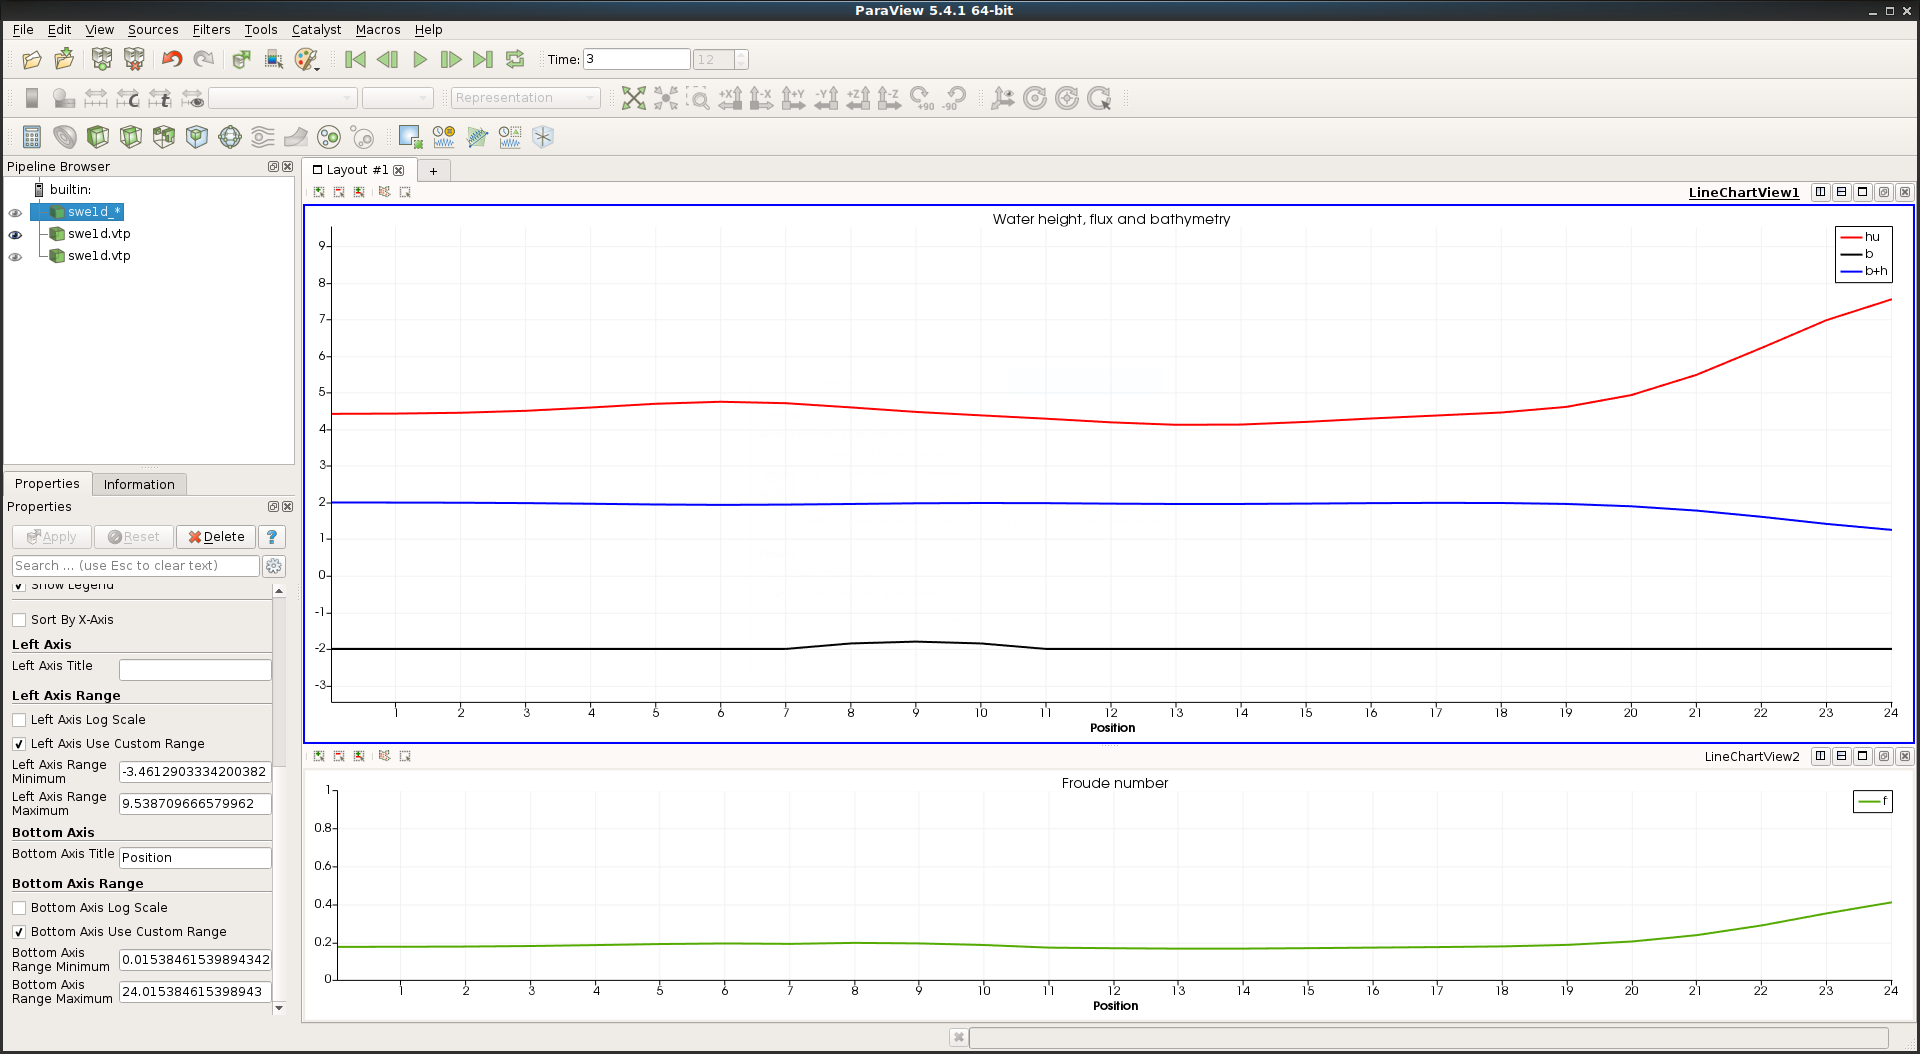
\includegraphics[clip, width=\imgfullscale\linewidth]{img/Subcritical.png}
	\end{figure}
	Critical section in range [7,9]\\
	Slightly increased froude number within the critical section
\end{frame}

\begin{frame}{Hydraulic jump: Supercritical scenario}
	\begin{figure}
		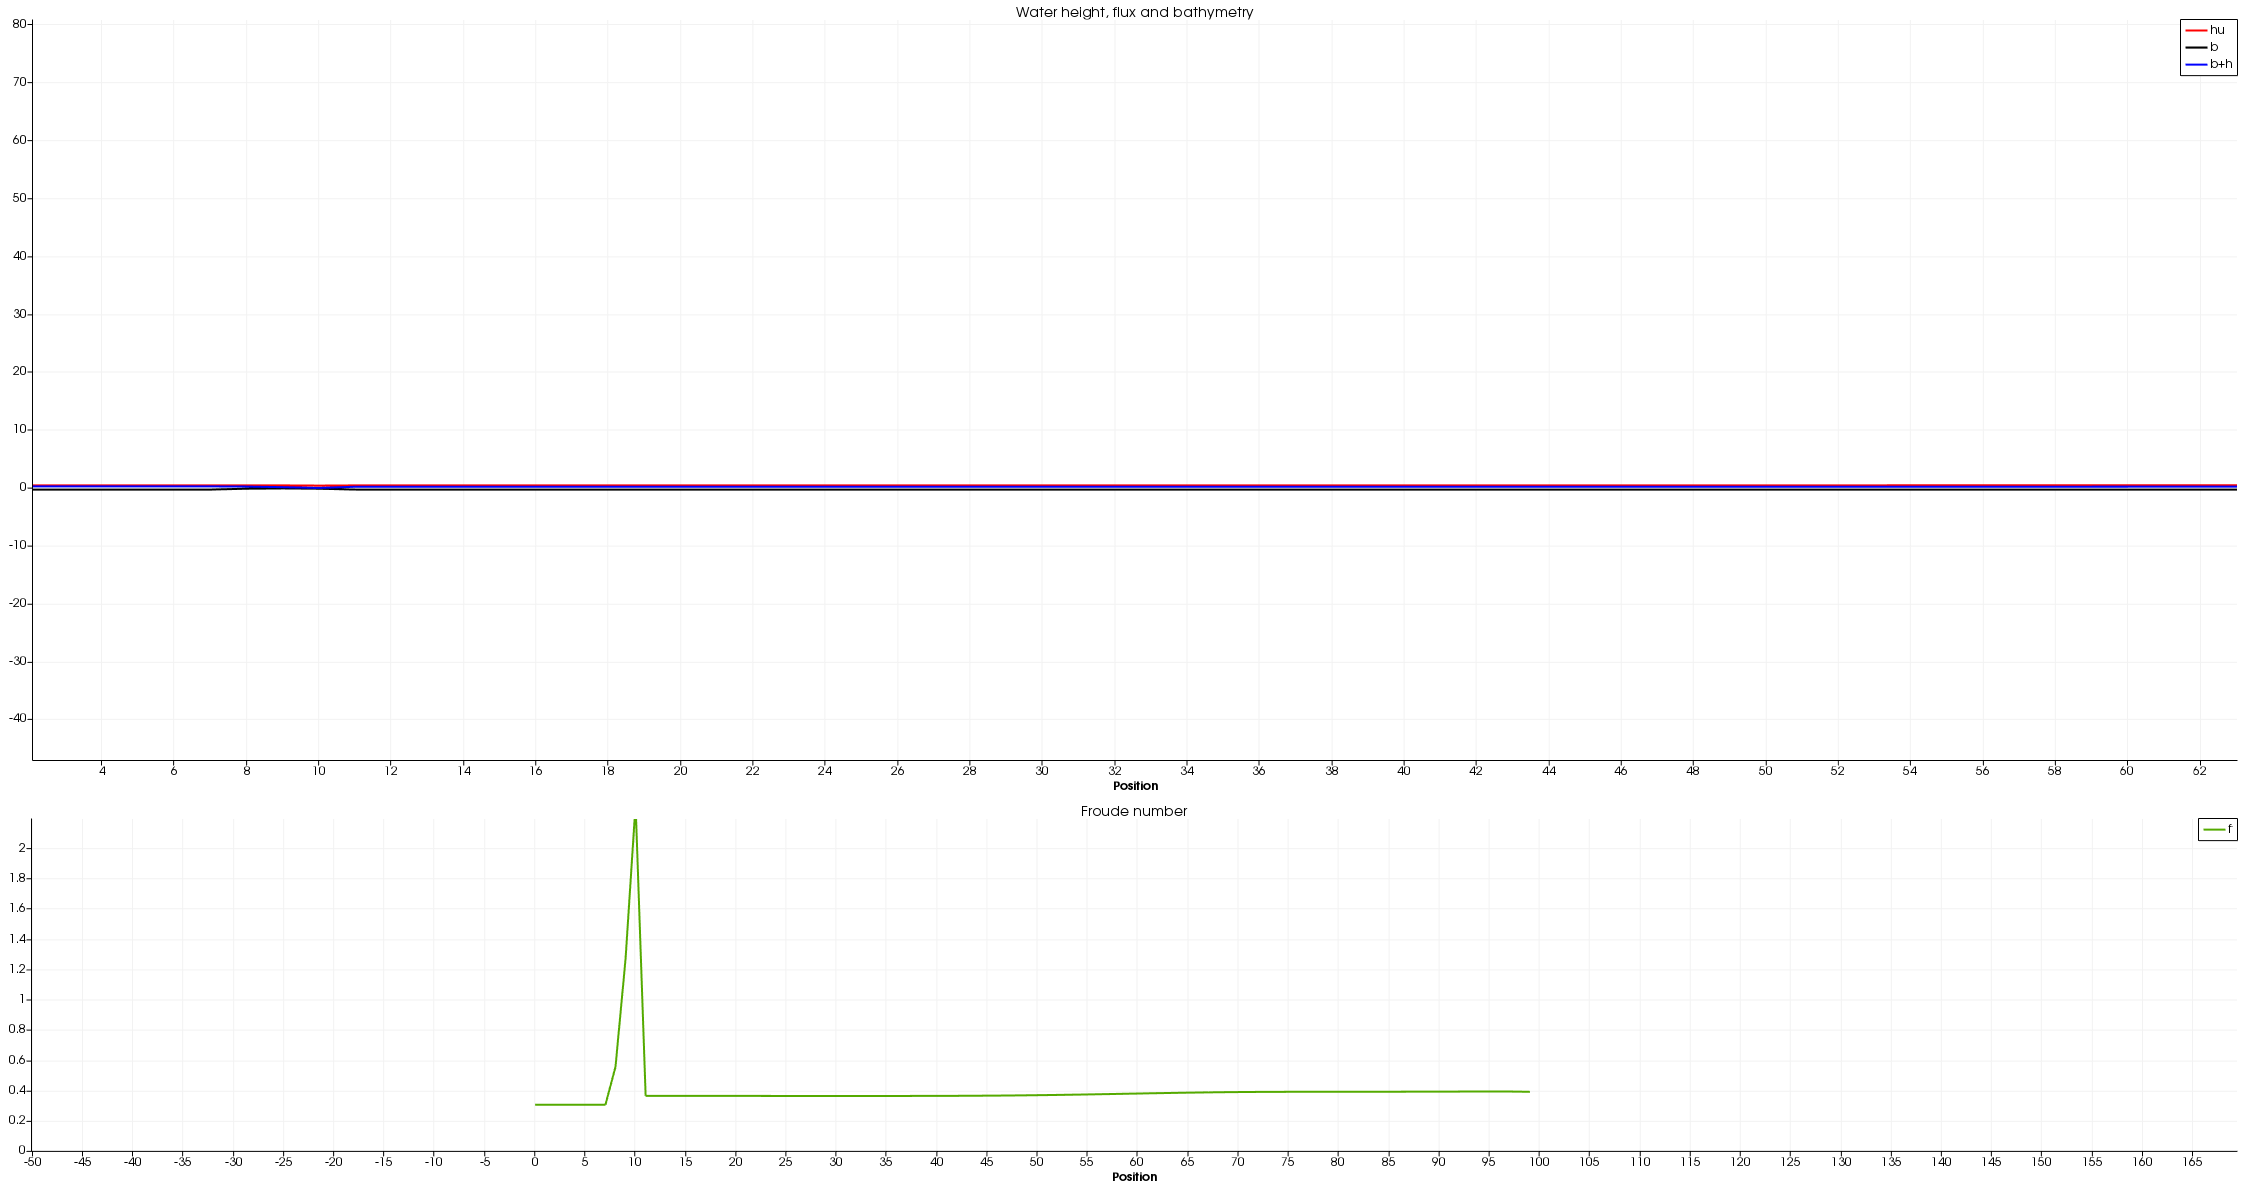
\includegraphics[clip, width=\imgfullscale\linewidth]{img/Supcritical.png}
	\end{figure}
	Some very nice text\\
	Position of stationary discontinuity
\end{frame}

\begin{frame}{Dimensional splitting: simple scenario}
	\begin{figure}
		
\includegraphics[clip, width=\imgfullscale\linewidth]{img/dummy_image.jpg}
	\end{figure}
	Some very nice text
\end{frame}

\begin{frame}{Dimensional splitting: extension of radial dam-break}
	\begin{figure}
		
\includegraphics[clip, width=\imgfullscale\linewidth]{img/dummy_image.jpg}
	\end{figure}
	Some very nice text
\end{frame}

\begin{frame}{}
	\begin{figure}
		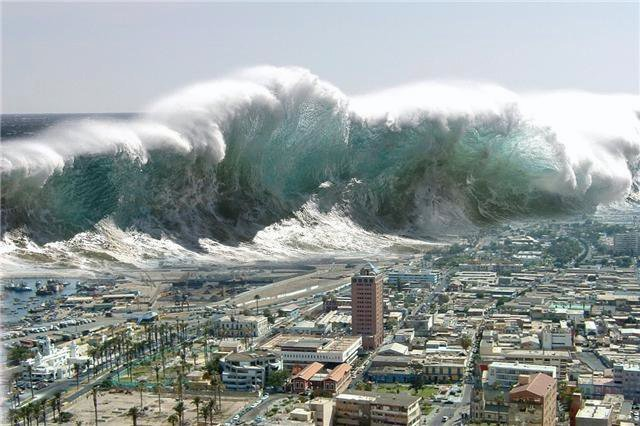
\includegraphics[clip, width=\imgfullscale\linewidth]{img/tsunami.jpg}
	\end{figure}
	\centering
	Thank you for your attention
	\\
	\vfill
	\flushleft
	{\fontsize{5}{5} \selectfont http://userscontent2.emaze.com/images/88c09d66-4283-49c0-9f80-9eb8fd05e30f/16101782-ea98-4b06-b114-4637be705926.jpg}
\end{frame}
\end{document}